\documentclass[tikz,border=3pt]{standalone}
\usepackage[utf8]{inputenc}
\usepackage[T1]{fontenc}
\usepackage{lmodern}
\renewcommand{\familydefault}{\sfdefault}
\usepackage{sansmath}\sansmath
\usepackage{chemfig}
\usepackage{pgfplots}\pgfplotsset{compat=1.18,/pgf/number format/use comma,/pgf/number format/1000 sep={.}}
\usetikzlibrary{arrows.meta,calc,positioning,decorations.pathmorphing,patterns}
% paleta del sitio
\definecolor{nar}{HTML}{E8680C}\definecolor{narc}{HTML}{FFB35C}\definecolor{hielo}{HTML}{FFF3E8}
\definecolor{tinta}{HTML}{1D1D1F}\definecolor{gris}{HTML}{6E6E73}\definecolor{lila}{HTML}{7C5CF0}
\definecolor{azul}{HTML}{2F6FD6}\definecolor{menta}{HTML}{17A673}\definecolor{coral}{HTML}{E8342A}
\begin{document}
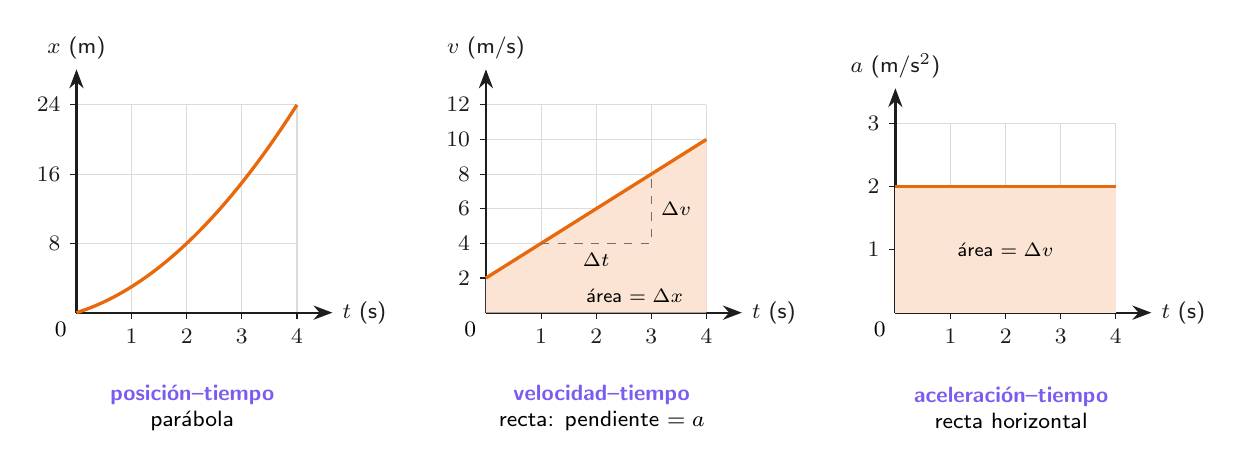
\begin{tikzpicture}[font=\footnotesize,>={Stealth[length=2.4mm]},]

\begin{scope}[x=0.7cm,y=0.11cm]
\draw[gris!25] (0,8) -- (4,8);
\draw[gris!25] (0,16) -- (4,16);
\draw[gris!25] (0,24) -- (4,24);
\draw[gris!25] (1,0) -- (1,24);
\draw[gris!25] (2,0) -- (2,24);
\draw[gris!25] (3,0) -- (3,24);
\draw[gris!25] (4,0) -- (4,24);
\draw[->,thick,tinta] (0,0) -- (4,0) -- ++(0.45cm,0) node[right] {$t$ (s)};
\draw[->,thick,tinta] (0,0) -- (0,24) -- ++(0,0.45cm) node[above] {$x$ (m)};
\draw[tinta] (1,0) -- ++(0,-0.08cm) node[below] {$1$};
\draw[tinta] (2,0) -- ++(0,-0.08cm) node[below] {$2$};
\draw[tinta] (3,0) -- ++(0,-0.08cm) node[below] {$3$};
\draw[tinta] (4,0) -- ++(0,-0.08cm) node[below] {$4$};
\draw[tinta] (0,8) -- ++(-0.08cm,0) node[left] {$8$};
\draw[tinta] (0,16) -- ++(-0.08cm,0) node[left] {$16$};
\draw[tinta] (0,24) -- ++(-0.08cm,0) node[left] {$24$};
\node[below left] at (0,0) {$0$};
\draw[very thick,nar,domain=0:4,smooth,variable=\t] plot (\t,{2*\t+\t*\t});
\node[align=center] at (2.1,-11) {\textbf{\color{lila}posición--tiempo}\\parábola};
\end{scope}
\begin{scope}[shift={(5.2cm,0)},x=0.7cm,y=0.22cm]
\draw[gris!25] (0,2) -- (4,2);
\draw[gris!25] (0,4) -- (4,4);
\draw[gris!25] (0,6) -- (4,6);
\draw[gris!25] (0,8) -- (4,8);
\draw[gris!25] (0,10) -- (4,10);
\draw[gris!25] (0,12) -- (4,12);
\draw[gris!25] (1,0) -- (1,12);
\draw[gris!25] (2,0) -- (2,12);
\draw[gris!25] (3,0) -- (3,12);
\draw[gris!25] (4,0) -- (4,12);
\draw[->,thick,tinta] (0,0) -- (4,0) -- ++(0.45cm,0) node[right] {$t$ (s)};
\draw[->,thick,tinta] (0,0) -- (0,12) -- ++(0,0.45cm) node[above] {$v$ (m/s)};
\draw[tinta] (1,0) -- ++(0,-0.08cm) node[below] {$1$};
\draw[tinta] (2,0) -- ++(0,-0.08cm) node[below] {$2$};
\draw[tinta] (3,0) -- ++(0,-0.08cm) node[below] {$3$};
\draw[tinta] (4,0) -- ++(0,-0.08cm) node[below] {$4$};
\draw[tinta] (0,2) -- ++(-0.08cm,0) node[left] {$2$};
\draw[tinta] (0,4) -- ++(-0.08cm,0) node[left] {$4$};
\draw[tinta] (0,6) -- ++(-0.08cm,0) node[left] {$6$};
\draw[tinta] (0,8) -- ++(-0.08cm,0) node[left] {$8$};
\draw[tinta] (0,10) -- ++(-0.08cm,0) node[left] {$10$};
\draw[tinta] (0,12) -- ++(-0.08cm,0) node[left] {$12$};
\node[below left] at (0,0) {$0$};
\fill[nar!18] (0,0) -- (0,2) -- (4,10) -- (4,0) -- cycle;
\draw[very thick,nar] (0,2) -- (4,10);
\node[font=\scriptsize] at (2.7,1.0) {área $= \Delta x$};
\draw[gris,dashed] (1,4) -- (3,4) -- (3,8);
\node[font=\scriptsize,right] at (3.0,6) {$\Delta v$};
\node[font=\scriptsize,below] at (2,4) {$\Delta t$};
\node[align=center] at (2.1,-5.5) {\textbf{\color{lila}velocidad--tiempo}\\recta: pendiente $= a$};
\end{scope}
\begin{scope}[shift={(10.4cm,0)},x=0.7cm,y=0.8cm]
\draw[gris!25] (0,1) -- (4,1);
\draw[gris!25] (0,2) -- (4,2);
\draw[gris!25] (0,3) -- (4,3);
\draw[gris!25] (1,0) -- (1,3);
\draw[gris!25] (2,0) -- (2,3);
\draw[gris!25] (3,0) -- (3,3);
\draw[gris!25] (4,0) -- (4,3);
\draw[->,thick,tinta] (0,0) -- (4,0) -- ++(0.45cm,0) node[right] {$t$ (s)};
\draw[->,thick,tinta] (0,0) -- (0,3) -- ++(0,0.45cm) node[above] {$a$ (m/s$^2$)};
\draw[tinta] (1,0) -- ++(0,-0.08cm) node[below] {$1$};
\draw[tinta] (2,0) -- ++(0,-0.08cm) node[below] {$2$};
\draw[tinta] (3,0) -- ++(0,-0.08cm) node[below] {$3$};
\draw[tinta] (4,0) -- ++(0,-0.08cm) node[below] {$4$};
\draw[tinta] (0,1) -- ++(-0.08cm,0) node[left] {$1$};
\draw[tinta] (0,2) -- ++(-0.08cm,0) node[left] {$2$};
\draw[tinta] (0,3) -- ++(-0.08cm,0) node[left] {$3$};
\node[below left] at (0,0) {$0$};
\fill[nar!18] (0,0) rectangle (4,2);
\draw[very thick,nar] (0,2) -- (4,2);
\node[font=\scriptsize] at (2,1) {área $= \Delta v$};
\node[align=center] at (2.1,-1.51) {\textbf{\color{lila}aceleración--tiempo}\\recta horizontal};
\end{scope}
\end{tikzpicture}
\end{document}
